\section{Background estimation}
\label{sec:htoinv_background_est}

% Here, give an overview of how the background estimation is done. Just say what the procedure is, generally, for each background

Accurate estimation of the \acrlong{sm} background processes in the signal region is paramount to a search for new physics. Mismeasured backgrounds and uncertainties can wash out traces of signal and affect the fit to data. The yields of the minor backgrounds are taken directly from simulation.\footnote{I guess this isn't really true if we group all backgrounds into Ttw and Zinv. In which case, will have to explain the grouping and reword stuff in this paragraph. So it may make sense to describe the fit before this, or integrate the background estimation section into it.} However, the lost lepton, invisibly decaying \PZ boson, and \acrshort{qcd} multijet processes must be predicted more carefully. The single lepton \glspl{CR} are used to constrain the lost lepton background, arising primarily from \ttbarpjets and \wtolnupjets. The dilepton and single photon \glspl{CR} predict the \ztonunupjets background. These processes rely on the \acrlong{mc} yields in those regions, and transfer factors arising from the \acrshort{mc} ratios between them and the signal region. Sidebands to the signal region estimate \acrshort{qcd} multijet contributions from data. The predicted background yields from each of these methods replace the \acrlong{mc} in the signal region when fed into the fit in Chpt.~\ref{sec:htoinv_satistical_treatment}. Fig.~\ref{fig:htoinv_fit_overview} illustrates the correspondence between the analysis regions and background predictions.

\begin{figure}[htbp]
    \centering
    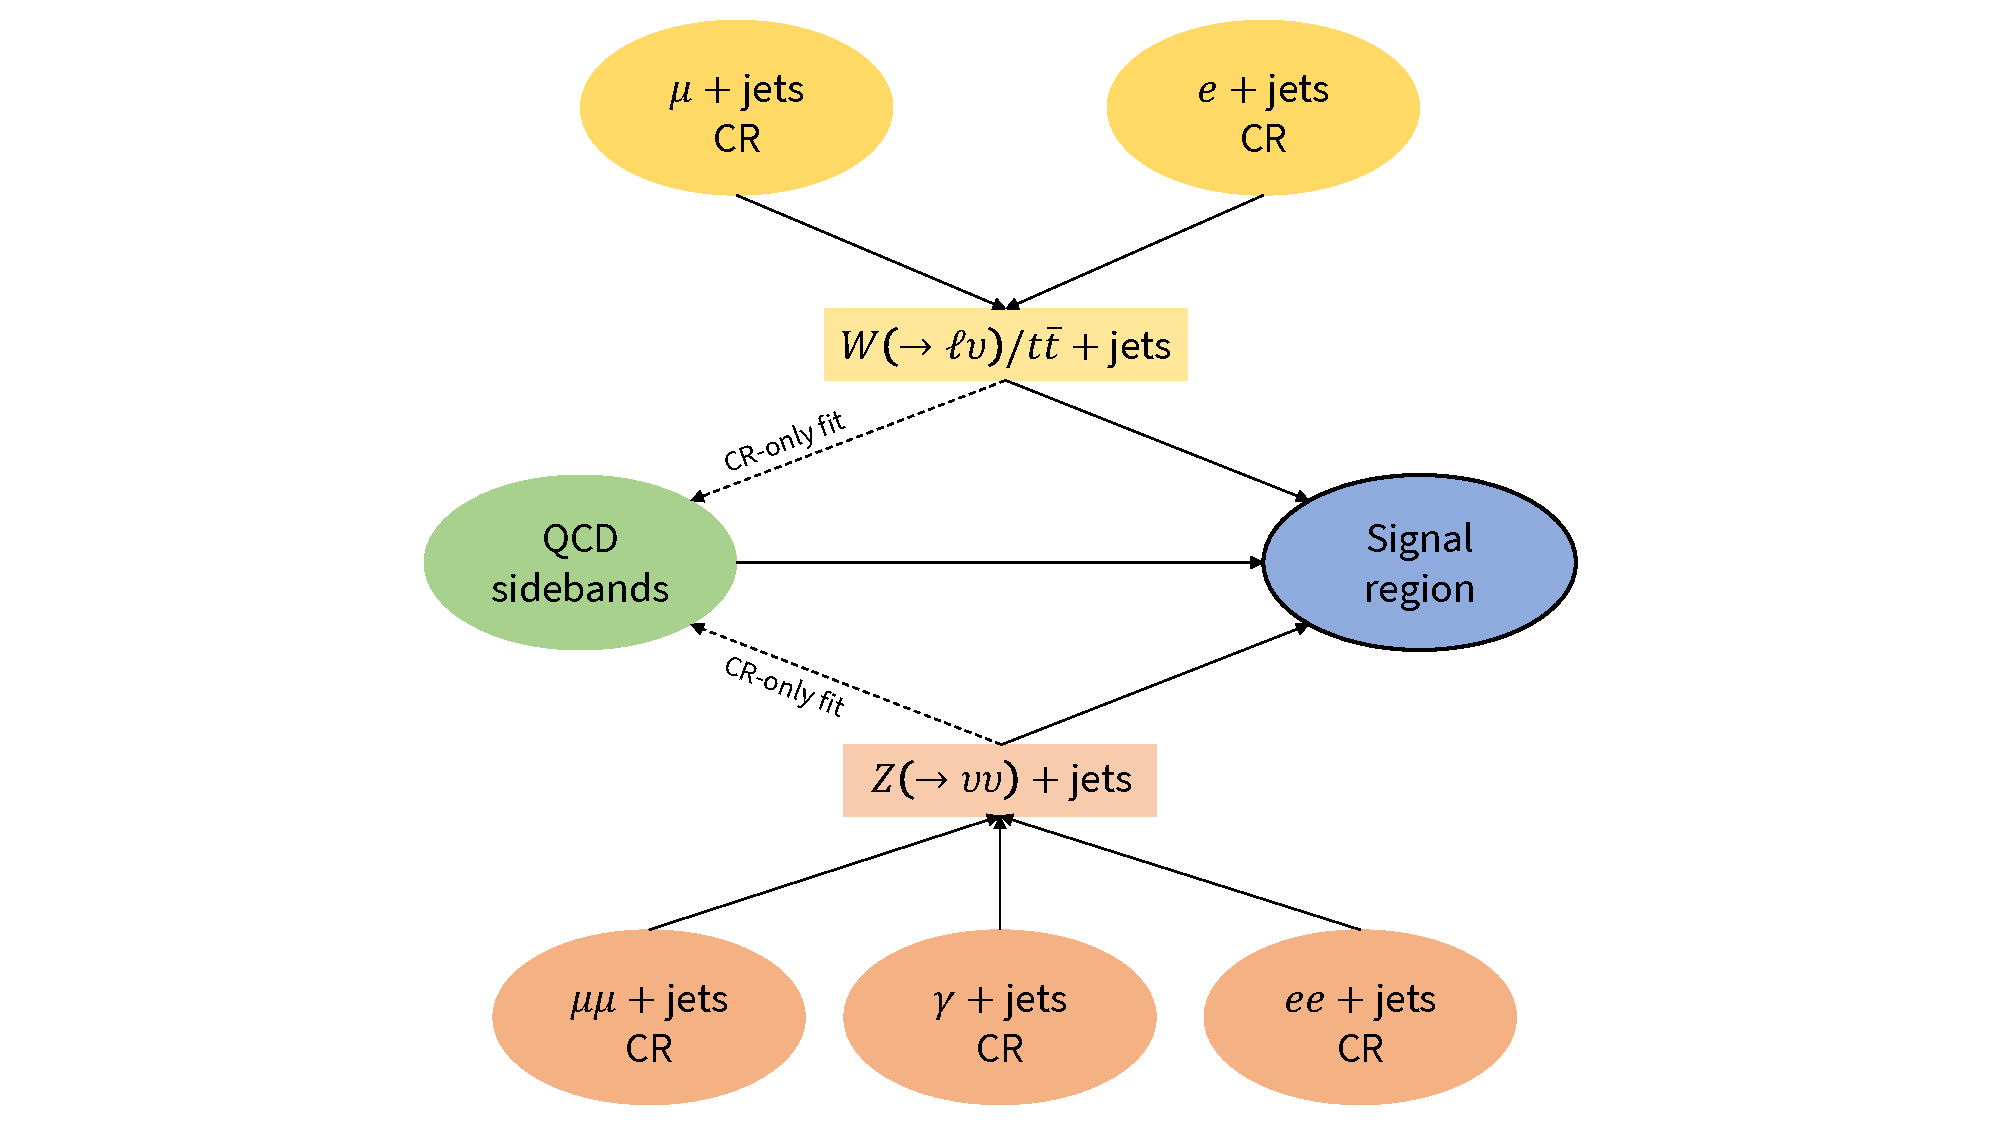
\includegraphics[width=0.5\textwidth]{figures/fit_overview.pdf}
    \caption[An infographic showcasing the role of each analysis region in the final fit]{An infographic showcasing the role of each analysis region in the final fit. The \glspl{CR} predict the lost lepton and \ztonunu backgrounds, and a \gls{CR}-only fit informs the \acrshort{qcd} multijet prediction that contributes to the eventual background determination in the signal region.}
    \label{fig:htoinv_fit_overview}
\end{figure}


%=========================================================


\subsection{Lost lepton (\texorpdfstring{\PW}{W} and \texorpdfstring{$\ttbarpjets$}{ttbar plus jets})}
\label{subsec:htoinv_lost_lepton_bkg}

In order to predict the lost lepton background in the signal region, a transfer factor $\transfac$ from simulation is defined that then scales the observed data in the single lepton \glspl{CR}. Events are categorised and binned in the same manner in the single lepton \glspl{CR} as in the signal region, such that the prediction is derived bin-by-bin. The transfer factor is simply the ratio of the simulation in the signal region to the \gls{CR}:
\begin{equation}
    \TF_{\singleMuCr} = \frac{ N_{\mathrm{MC}}^{\lostlepton, \, \mathrm{SR}}(\mathrm{subcategory}, \, \ptmiss) }{ N_{\mathrm{MC}}^{\singleMuCr}(\mathrm{subcategory}, \, \ptmiss) }
\end{equation}

The predicted yield in the signal region is then
\begin{equation}
    N_{\mathrm{pred.}}^{\lostlepton}(\mathrm{subcategory}, \, \ptmiss) = \TF_{\singleMuCr} \cdot N_{\mathrm{data}}^{\singleMuCr}(\mathrm{subcategory}, \, \ptmiss)
\end{equation}

% How is this modified when electrons are used as well?


%=========================================================


\subsection{\texorpdfstring{\ztonunupjets}{Z to nunu + jets}}
\label{subsec:htoinv_znunu_bkg}


%=========================================================


\subsection{QCD multijet}
\label{subsec:htoinv_qcd_multijet_bkg}

The effects of \gls{jet} mismeasurements are difficult to quantify. With a final state of several \glspl{jet} in the \acrshort{qcd} multijet process, low, or even no, \ptvecmiss is expected. Therefore, a single mismeasured \gls{jet} will introduce artificial \ptvecmiss in the direction of that jet. A low $\mindphiAB{\mathrm{j}}{\ptvecmiss}$ is therefore expected. Though it is not just this process that suffers---\glspl{jet} from ``cleaner'' processes may also be affected---those with real \ptmiss in an event (e.g., $\ztonunupjets$) are unlikely to be significantly affected by one stray object. The enormous cross section of \acrshort{qcd} multijet also amplifies the problem, making the process as a whole more sensitive to, e.g., fluctuations in the calorimeter response that would affect the energy measurement.

Contributions to the signal region from \acrshort{qcd} multijet events should be adequately suppressed by the analysis-level selection requirements. However, it is still a process that must be accurately accounted for considering its rate of production at \acrshort{cms}. A metric by which to estimate the number of events a dataset should require is by calculating the equivalent luminosity:
\begin{equation}
    \lumi_{\mathrm{eq.}} = \frac{N_{\mathrm{events}}}{\sigma}
    \label{eq:equivalent_lumi}
\end{equation}

A general rule is that the equivalent luminosity of a given dataset should be comparable to, or even exceed, that of the data collected by the experiment. Since the \acrshort{qcd} multijet process has a very large cross section, simulating the required number of events to match the luminosity of the data recorded during Run-2 is not feasible. This can be mitigated by using a data-driven method to estimate it from the multijet-enriched sidebands described in Chpt.~\ref{subsec:htoinv_sidebands}.

To estimate the presence of \acrshort{qcd} in the signal region, a data driven approach is taken utilising the sidebands defined in Chpt.~\ref{subsec:htoinv_sidebands}. These are derived separately for each category and data taking year. Firstly, a fit to the lepton and photon \glspl{CR} is performed to extract the rate parameters that scale the non-multijet background in each subcategory and \ptmiss bin. Applying these scale factors to the relevant backgrounds in the sidebands changes the distribution and hence the data/\acrshort{mc} agreement. The excess in data in a sideband is assumed to arise solely from multijet events, and as such the difference between data and the non-multijet background is attributed to \acrshort{qcd} (denoted as $N_{\mathrm{SB}}^{\mathrm{QCD}}$).

\acrshort{qcd} in the signal region $N_{\mathrm{pred.}}^{\mathrm{QCD}}$ is predicted in each subcategory and \ptmiss bin as follows: 
\begin{equation}
    N_{\mathrm{pred.}}^{\mathrm{QCD}}(\mathrm{subcategory}, \, \ptmiss) = N_{\mathrm{SB}}^{\mathrm{QCD}} \cdot \transfac_{\mathrm{QCD}} \cdot \catFraction(\mathrm{subcategory}) \cdot \metFraction(\ptmiss)
    \label{eq:qcd_prediction}
\end{equation}

% Explaining the TF sounds a bit weird, but will hopefully make more sense once I've explained the transfer factors for the lost lepton and Z->invisible prediction as they're bin-by-bin
where $\transfac_{\mathrm{QCD}}$ is the transfer factor relating the \acrshort{qcd} in the sideband to the multijet simulation in the signal region. As the signal region is depleted in simulated multijet events, the transfer factor is inclusive over the region rather than per \ptmiss bin and subcategory, i.e.,
\begin{equation}
    \transfac_{\mathrm{QCD}} = \frac{ N_{\mathrm{MC, \ SR}}^{\mathrm{QCD}} } { N_{\mathrm{MC, \ SB}}^{\mathrm{QCD}} }
%   \transfac_{\mathrm{QCD}} = \frac{ \sum_{\mathrm{subcategory}, \, \ptmiss}^{\mathrm{SR}} N_{\mathrm{MC}}^{\mathrm{QCD}}(\mathrm{subcategory}, \, \ptmiss) }{ \sum_{\mathrm{subcategory}, \, \ptmiss}^{\mathrm{SB}} N_{\mathrm{MC}}^{\mathrm{QCD}}(\mathrm{subcategory}, \, \ptmiss) }
    \label{eq:transfer_factor_qcd}
\end{equation}

The distribution of the \acrshort{qcd} background for each subcategory and \ptmiss bin is extrapolated from the sidebands with the factors $\catFraction$ and $\metFraction$. $\catFraction$ is the fraction of \acrshort{qcd} in a given subcategory of a given sideband, inclusive of \ptmiss. For the \ttH and \ggH categories, the tight double sideband from Tab.~\ref{tab:sideband_defs}---the most enriched in \acrshort{qcd} \acrshort{mc}---is used to derive the factor. $\metFraction$ is the fraction of \acrshort{qcd} in a given \ptmiss bin of a given sideband, inclusive of subcategory. For the \ttH and \ggH categories, the loose double sideband is used to derive the factor. This sideband is used for the prediction as a whole, i.e., for the terms $N_{\mathrm{SB}}^{\mathrm{QCD}}$ and $\transfac_{\mathrm{QCD}}$ in Eq.~\ref{eq:qcd_prediction}.

% Need to mention how prediction is done for VH, given sidebands 0 and 2 are pretty depleted in stats. Also need to mention how uncertainty is handled for the predicted QCD
